\documentclass{article}

\usepackage{graphicx}

\title{Writing Assignment 1}
\author{Qi Mao\\
  \texttt{maoxx241@umn.edu}}
\maketitle


\begin{document}
I think the App used in the story could be created using our current technology.
Actually, we already have a similar feature app. 


In China, there is an app named Bi Xin.
This app is used to find people who have a high-rank level or have a pretty face or have a sweet sound
to play computer games face to face.
The whole process is straightforward. You only need to publish an order to specify your requirements.
Then the app will post the order to someone nearby who meets the requirements.
If some people think that your the requirements and the price is appropriate
, then he or she will confirm the order and meet at the agreed location (usually an internet cafe nearby).


Here are some screenshots of the Bi Xin app.
\begin{center}
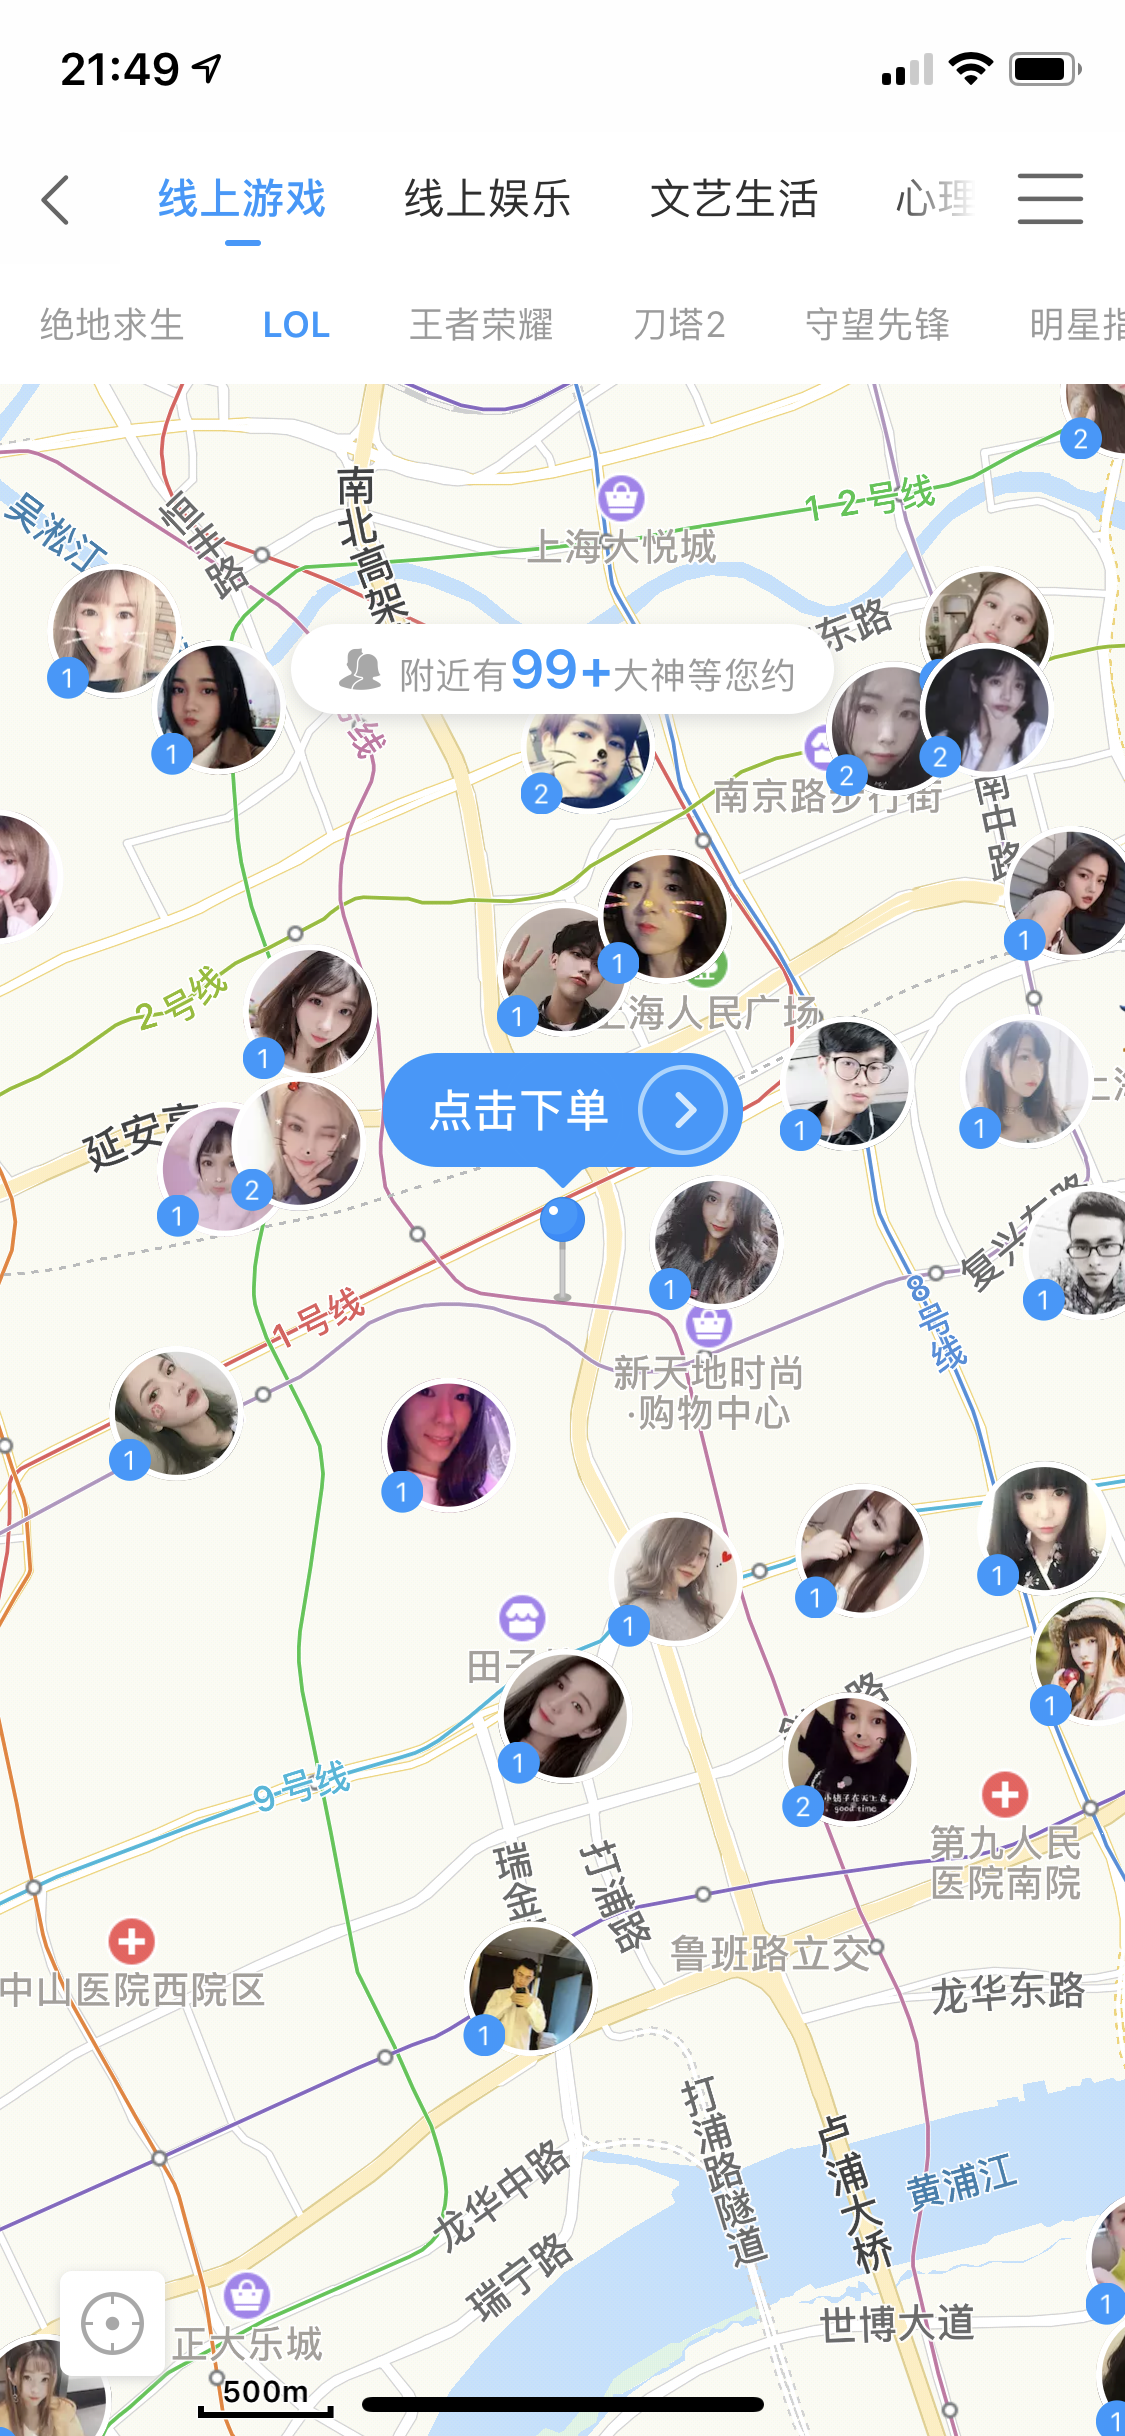
\includegraphics[scale=0.09]{IMG_5883}
\end{center}

You can click on the picture on the map to find nearby people.
\newpage

\begin{center}
  \includegraphics[scale=0.09]{IMG_5884}
  
\end{center}
the blue button means order now and play with him is 10 RMB each game.
\\
\\

I think this app is very similar to the app in the article, but the app in the article is more used to get information,
 Bi Xin is more used to find the people around to play games.It is worth mentioning that although this App is used to find people to play games. 
There are also many people who use Bi Xin to get the information they want, such as nearby food, attractions, and even looking for pretty girls.
The most significant difference between the two apps is that the third party's subject is different when the order is executed.
The third party body of the app in the article can be any information about anyone, but the third party in Bi Xin is just a computer game.
This is the most fundamental difference between the two apps.

I think Bi Xin is the app in this fiction story that implements a part of functions.
If the app described in the paper were available, I would use it.
Because this app will help me a lot.
If I feel that playing games alone is boring,
then I can use this app to find an interested person to play games with me.
If I want to know if the steak in Cub is fresh or not,
I can find someone to help me without going out.
Using money to save time is a very cost-effective thing.


Some of Aaron's actions are ethical.
 Once, he found a little girl separated from her parents in the mall, 
 which was good and ethical,
  because it made both little girl and her parents happy. Moreover, 
  Aaron shared the information about whether the seats in the coffee shop are free or not. 
  Aaron took some photos in the museum and send them to others.


There are three main things about Aaron's unethical behavior: 



\begin{center}
  \begin{tabular}{ |l|l|}
    \hline
    ethical behavior & unethical behavior  \\ \hline
    Find the little girl & take photos of the manager's special dustbin  \\ \hline
    shared the information & filmed two women kissing on a video\\
    about the coffee shop &   \\ \hline
    took photos in the museum & shot the license plate number of his father's car \\
    \hline
  \end{tabular}
\end{center}


At first, Aaron went to the supermarket to take photos of the manager's special dustbin. 
Although it was a dustbin, if the manager knew about it, 
he would feel uncomfortable, so I think it is not good.
 The second time is Aaron went to a dimly lit bar and filmed two older women kissing on a video.
  Aaron then showed the video to a peeper and Aaron got a reward. 
  I think Aaron was violating other people's privacy.
   In the third scene, Aaron shot the license plate number of his father's car and betrayed his father. 
   After he provided information to others, he did it without his father's permission, 
   so it was unethical.

  
The essence of this app is to use time to exchange someone else's time plus information.
The unethical behavior mentioned in the article merely violates the privacy rights of third parties.
We can expect terrorists to use this app to learn about the time and place of the police patrol.
They only need to spend money to hire people who need to make money with this app, 
and then pay a small amount of dollars.
\end{document}